\chapter{Justificación}

Los estudios de nueva física, en particular los que predicen la producción de nuevas partículas, son bastantes relevantes dado que se aproxima la etapa de alta luminosidad del Gran Colisionador de Hadrones en donde se logrará acumular datos con una frecuencia 10 veces mayor en la que se estaba operando. Lo anterior indica que la probabilidad de detección de nuevas señales será mucho mayor ya que se logrará alcanzar un rango de energía mayor y una cantidad de datos igualmente superior. Usualmente la probabilidad de producción de estas partículas exóticas es baja por lo que se requiere de una cantidad grande de datos para poder observar dicha producción. El período de alta luminosidad está programado para empezar a partir del año 2024 o 2025, como se puede ver en al línea de tiempo del Gran Acelerador de Hadrones en la Figura \ref{fig:LHC_timeline}, sin embargo desde este momento se está trabajando en la actualización del detector, en métodos de análisis y en estrategias que ayuden a optimizar la búsqueda de nueva física.

\begin{figure}
    \centering
    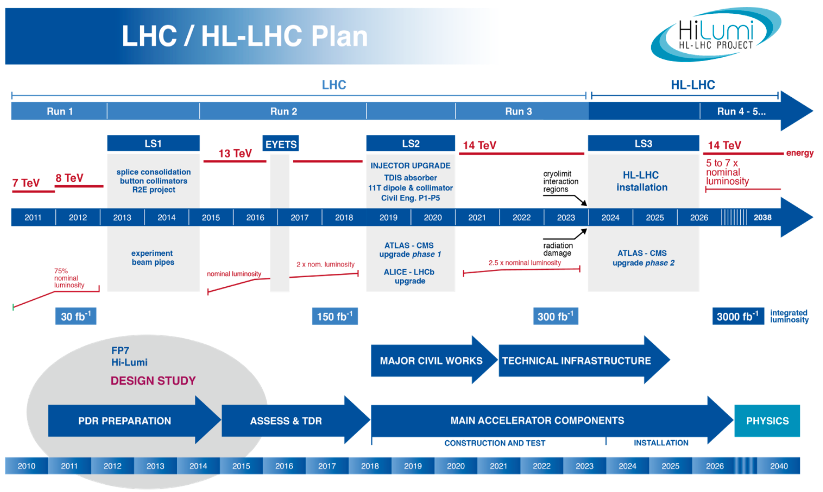
\includegraphics[width=0.84\textwidth]{JUSTIFICACION/LHC_timeline.png}
    \caption{Agenda de actividades del Gran Colisionador de Hadrones, donde la fase de alta luminosidad está programada para iniciar a partir del 2024-2025.}
    \label{fig:LHC_timeline}
\end{figure}

Actualmente los modelos teóricos que predicen la formación de partículas de materia oscura no han sido explorados ampliamente, en gran medida por falta de datos experimentales que permitan alcanzar el espacio fase que dichos modelos predicen para esas partículas. Por todo ello el funcionamiento del Gran Acelerador de Hadrones y sus proyecciones en cuanto a recolección de datos en los próximos años constituye una oportunidad perfecta para explotar con mayor intencionalidad el estudio de dichos modelos en aras de descubrir una nueva señal de fácil interpretación en el contexto de los modelos propuestos. 


